\documentclass[12pt]{article}
\usepackage{lmodern} % Pour une police plus nette
\usepackage{stmaryrd}
\usepackage{graphicx} % Pour l'insertion d'images
\usepackage{float}    % Pour contrôler précisément le placement
\usepackage[utf8]{inputenc}
\usepackage[french]{babel}
\usepackage[T1]{fontenc}
\usepackage[colorlinks=true, linkcolor=blue, urlcolor=blue, citecolor=blue]{hyperref}
\usepackage{verbatim}
\usepackage{color, soul}
\usepackage{pgfplots}
\pgfplotsset{compat=1.18} % Version plus récente de pgfplots
\usepackage{mathrsfs}
\usepackage{amsmath}
\usepackage{amsfonts}
\usepackage{amssymb}
\usepackage{tkz-tab}

%\author{Destiné aux élèves de Terminale S\\Lycée de Dindéfelo\\Présenté par M. BA}
%\title{\textbf{Rappels et compléments sur les fonctions numériques}}
%\date{\today}
\usepackage{tikz}
\usetikzlibrary{arrows, shapes.geometric, fit}
% Commande pour la couleur d'accentuation
\newcommand{\myul}[2][black]{\setulcolor{#1}\ul{#2}\setulcolor{black}}
\newcommand\tab[1][1cm]{\hspace*{#1}}
\usepackage[margin=2.5cm]{geometry} % Ajustement des marges
\usepackage{eso-pic} % Pour ajouter des éléments en arrière-plan

% Commande pour ajouter du texte en arrière-plan, centré au milieu de chaque page
\AddToShipoutPicture{
    \AtPageCenter{%
        \makebox(0,0)[c]{\rotatebox{60}{\textcolor[gray]{0.9}{\fontsize{2cm}{2cm}\selectfont Pathé Gobel BA}}}
    }
}

\begin{document}

\noindent
\begin{minipage}[t]{0.48\textwidth}
\raggedright
\textbf{Ministère de l'Éducation Nationale}\\
Inspection Académique de Kédougou\\
Lycée Dindéfelo\\
Cellule de Mathématiques
\end{minipage}
\hfill
\begin{minipage}[t]{0.48\textwidth}
\raggedleft
\textbf{Année scolaire 2024-2025}\\
Date : 17/10/2024\\
Classe : Terminale S2\\
Professeur : M. BA
\end{minipage}

\vspace{1cm}
\section*{Exercice 1}

1. Déterminer, si elles existent, les limites suivantes :

\[
\lim_{x \to 0} \frac{\tan(3x)}{1 - \sqrt{x + 1}} \quad ; \quad \lim_{x \to 2} \frac{\sqrt{x+2} - \sqrt{3x+3}}{x-2} \quad ; \quad \lim_{x \to 0} \frac{\cos x - 1}{x^3 + x^2}
\]

\[
\lim_{x \to 0} \frac{3 \sin^2 x - \cos x + 1}{x^2} \quad ; \quad \lim_{x \to 0} \frac{\sin x - \tan x}{x^3}\quad ; \quad\lim_{x \to 0} \frac{1 - \cos x}{x \tan x}
\]

2. Déterminer, si elles existent, les limites suivantes :

\[
\lim_{x \to \frac{\pi}{2}} \frac{1 - \tan x}{1 + \tan x}\quad ; \quad \lim_{x \to 3} \frac{\sqrt{x+1} - 2}{\sqrt{x^2 - x - 6}}\quad ; \quad\lim_{x \to 1} \frac{\sqrt{x+3} - \sqrt{5-x}}{\sqrt{2x+7} - \sqrt{10-x}}
\]
\[
\lim_{x \to 0} \frac{\sqrt{1+\sin x} -1}{\sin 2x}\quad ; \quad\lim_{x \to \frac{\pi}{2}} \frac{\cos x}{1-\sin x}
\]

3. Déterminer, si elles existent, les limites suivantes :

\[
\lim_{x \to \pm \infty} \left(x - \sqrt{x^2 + 3x - 1}\right)\quad; \quad \lim_{x \to \pm \infty} \frac{2x + \sqrt{x^2 + 1}}{x}\quad; \quad
\lim_{x \to \pm \infty} \frac{x+1}{\sqrt{x+3}-2}
\]

\[
\lim_{x \to \pm \infty} \left(2x + \sqrt{x - 1}\right)\quad; \quad
\lim_{x \to \pm \infty} \left(x + \sqrt{2x^{2} - 5x + 1 }\right)\quad; \quad
\lim_{x \to \pm \infty} \left(x\sqrt{\frac{x+1}{x-1}}\right)
\]

\[
\lim_{x \to \pm \infty} \frac{x - \sqrt{|x|}}{3x + 2}
\]

\[
\lim_{x \to +\infty} \sqrt{5x-2}-\sqrt{x+1}
\]
4. Déterminer, si elles existent, les limites suivantes :
\[
\lim_{x \to \pm \infty} \frac{x^2 + \sin x}{x} \quad ; \quad \lim_{x \to \pm\infty} \frac{x + \sin x}{2 - \sin x} \quad ; \quad \lim_{x \to \pm \infty} \frac{x^3}{3 + 2 \sin x}
\]

5. Déterminer les réels \( a \) et \( b \) pour que la droite d'équation \( y = ax + b \) soit une asymptote à la courbe représentative de la fonction \( x \mapsto \sqrt{x^2 + 4} - \frac{x}{\sqrt{2}} \).

\section*{Exercice 2}

Calculer les limites suivantes :

\[
1. \quad \lim_{x \to \frac{\pi}{4}} \frac{2 \cos x - \sqrt{2}}{x - \frac{\pi}{4}} \quad ; \quad \lim_{x \to 1} \frac{\sin(\pi x)}{x - 1}
\]

\[
2. \quad \lim_{x \to \frac{\pi}{4}} \frac{1 - \sqrt{2} \cos x}{1 - \sqrt{2} \sin x} \quad ; \quad \lim_{x \to 0^+} \frac{x \cos x + \sin x}{\sqrt{x + 1} - 1} \\
\]
\[
3. \quad \lim_{x \to \frac{\pi}{4}} \frac{\tan x - 1}{x - \frac{\pi}{4}} \quad ; \quad \lim_{x \to 0} \frac{1}{x^2} \left( \frac{2}{\cos x }+ \cos x - 3 \right)
\]
\[
4. \quad \lim_{x \to +\infty} \left( x \arctan (\sqrt{x}) - \frac{\pi}{2} x \right) \quad ; \quad \lim_{x \to 0^+} \frac{1}{x} \arctan \left( \frac{\sqrt{x}}{x + 1} \right)
\]

\[
5. \quad \lim_{|x| \to +\infty} \left( 3x - 1 + \sqrt{9x^2 + 3x - 2} \right) \quad ; \quad \lim_{x \to 0} \frac{1 - x^2 E \left( \frac{1}{x} \right)}{1 + x^2 E \left( \frac{1}{x} \right)} 
\]

\section*{Exercice 3}

Étudier la continuité de la fonction $f$ sur $D_f$ dans chaque cas.

1. $f(x) = x + \sqrt{x+1}$.

2. $f(x) = 4x + 1 + \frac{1}{x - 1}$.

3. $f(x) = 2\sqrt{x} - x$.

4. $f(x) = \frac{\sqrt{1 + x}}{1 - x}$.

\section*{Exercice 4}


Donner la dérivée des fonctions définies par :

\[
f(x) = \frac{1 + \cos(2x)}{1 - \sin(2x)} \quad ; \quad
g(x) = \left( x + \frac{1}{x} \right) \sqrt{\frac{1}{x}} \quad ; \quad
h(x) = \sqrt[3]{x - 6} + \frac{1}{x} \quad ; \quad
k(x) = \left| \frac{x^2 - x}{x - 1} \right|
\]

\[
m(x) = x \sqrt{\frac{x^2 - 1}{x^2 + 1}} \quad ; \quad
n(x) = \frac{\sqrt{x^2 - 3x + 2}}{x + 1} \quad ; \quad
p(x) = \frac{\tan x}{1 - 2 \sin x}
\]

\[
q(x) = 3 \left( x^2 - 3x + 5 \right)^4 \quad ; \quad
r(x) = \cos^2(3x) \quad ; \quad
s(x) = -2 \tan^2(2x)
\]
\newpage
\section*{Exercice 5}
Etude d'une fonction par lecture graphique
\begin{figure}[h]
\centering
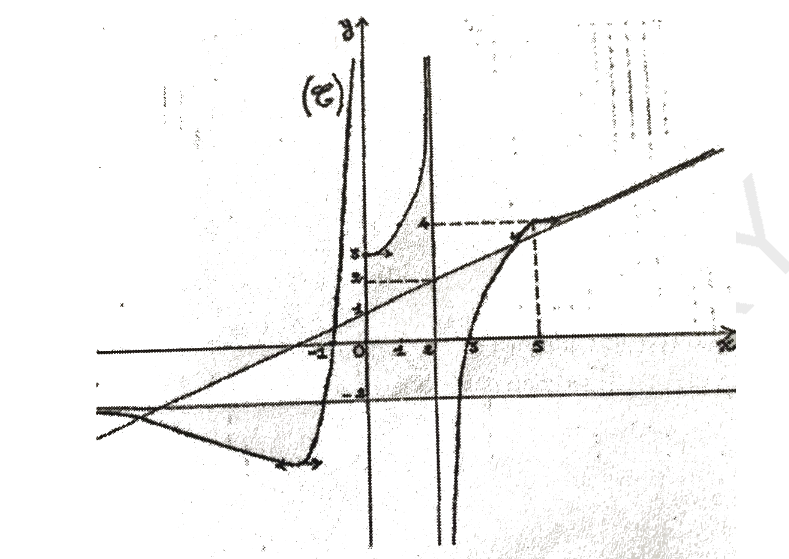
\includegraphics[width=0.8\textwidth]{courbe.png}
\caption{Courbe de (Cf)}
\label{fig:monimage}
\end{figure}
%\includegraphics[scale=0.8]{c1c2c3.png}
La courbe $(C_f)$ ci-dessus est celle d'une fonction $f$ dans un repère orthonormé. $f$ est définie en 0 et on a : $f(0) = 3$.

\begin{enumerate}
    \item Préciser l'ensemble de définition de $f$.
    \item Donner les limites suivantes :
    \[
    \textbf{a)} \lim_{x \to +\infty} f(x), \quad \lim_{x \to -\infty} f(x) ;
    \]
    \[
    \textbf{b)} \lim_{x \to 0^+} f(x), \quad \lim_{x \to 0^-} f(x) ;
    \]
    \[
    \textbf{c)} \lim_{x \to 2^+} f(x), \quad \lim_{x \to 2^-} f(x) ;
    \]
    \item La courbe admet-elle une asymptote oblique ? Si oui, donner son équation.
    \item Préciser les équations des autres asymptotes.
    \item La fonction $f$ est-elle dérivable en 5 ? Justifier la réponse.
    \item Dresser le tableau de variation de $f$.
\end{enumerate}

\section*{Exercice 6}

Le tableau de variation ci-dessous est celui d'une fonction $f$ continue sur son ensemble de définition avec $f'(1) = 0$ et $f'(4) = -1$. La courbe $(C_f)$ de $f$ coupe l'axe des abscisses en $A(-2;0)$ et $B\left(-\frac{1}{2};0\right)$ et l'axe des ordonnées au point $C(0;2)$.

La droite $(D) : y = x - 3$ est une asymptote oblique en $+\infty$ et est en dessous de $(C_f)$ sur $[0; +\infty[$.

    \begin{tikzpicture}[node style/.style={fill opacity=0,text opacity=1}]
        \tkzTabInit[espcl=1.75]{$x$/.5,$f'$/.7,$f$/1.5}{$-\infty$,$-3$,$-1$,$1$,$3$,$+\infty$}
        \tkzTabLine{,-,z,+,d,+,z,-,z,+,}
        \tkzTabVar{+/$-1$,-/$-3$,+D-/$+\infty$/$-\infty$,+/$4$,-/$2$,+/$+\infty$}
    \end{tikzpicture}

\begin{enumerate}
    \item Déterminer le domaine de définition de $f$ puis donner les limites aux bornes.
    \item Déterminer le domaine de dérivabilité de $f$.
    \item Déterminer en justifiant toutes les asymptotes à la courbe de $f$.
    \item Donner l'équation de chacune des demi-tangentes à la courbe au point d'abscisse 1.
    \item Tracer $(D)$ et $(C_f)$ dans un repère orthonormé d'unité 1 cm.
    \item Soit $g$ la restriction de $f$ à l'intervalle $[3; +\infty[$.
    \begin{enumerate}
        \item $g$ est-elle bijective ? Justifier.
        \item $g^{-1}$ est-elle dérivable en 2 ? Justifier.
    \end{enumerate}
    \item Graphiquement, déterminer l'ensemble des valeurs de $m$ pour lesquelles l'équation $f(x) = m$ admet exactement 4 solutions réelles distinctes.
\end{enumerate}
\section*{Exercice 7}

Soit $f$ la fonction donnée par : $f(x) = \frac{2 \sin(2x)}{1 + \cos(x)}$

\begin{enumerate}
    \item Déterminer le domaine de définition de $f$ puis montrer qu’on peut réduire le domaine d’étude de $f$ à l’intervalle $]0, 2\pi[$.
    \item Déterminer la limite de $f$ en $\pi$.
    \item Soit $\alpha$ l’unique réel de $]0, 2\pi[$ tel que $\cos(\alpha) = \frac{-1 + \sqrt{5}}{2}$. Montrer que $\cos(2x) + \cos(x) - 1 > 0$ si et seulement si $x \in ]0, \alpha[$.
    \item Montrer que $f'(x) = \frac{4( \cos^2(2x) + \cos(x) - 1)}{1 + \cos(x)}$, en déduire le signe de $f'(x)$ en utilisant (3), puis dresser le tableau de variation de $f$ sur $]0, 2\pi[$.
    \item Tracer la courbe de $f$ sur $]-2\pi, 2\pi[$. Unité : 1 cm.
\end{enumerate}

\section*{Problème n°1}

Soit la fonction numérique  f : $\mathbb{R} \to \mathbb{R}$  définie par :
\[
f(x) =
\begin{cases}
-x + 2 - \frac{2x}{x^2 + 1} & \text{si } x \leq 1, \\
x - 1 - 3\sqrt{x^2 - 1} & \text{si } x > 1.
\end{cases}
\]

\subsection*{Partie A}

\begin{enumerate}
    \item Justifier que $D_f = \mathbb{R}$.
    \item Étudier la continuité et la dérivabilité de $f$ en $x_0 = 1$.
    \item Iterpréter les résultats obtenus
    \item Déterminer les limites de $f$ aux bornes de $D_f$.
    \item (a) Montrer que la courbe $(C_f)$ admet deux asymptotes $(D_1)$ et $(D_2)$ à préciser.
\end{enumerate}
\begin{enumerate}
    \item[(b)] Préciser la position de \( (C_f) \) par rapport à \( (D_1) \) et \( (D_2) \).
\end{enumerate}

\begin{enumerate}
    \item[5.] (a) Calculer \( f'(x) \) dans les intervalles où \( f \) est dérivable (justifier l’existence de ces dérivées).
    \item[(b)] Établir le tableau de variations de \( f \).
    \item[(c)] Tracer \( (C_f) \) et les asymptotes dans un repère orthonormé \( (O; \vec{i}, \vec{j}) \).
\end{enumerate}
\subsection*{Partie B}

Soit \( g \) la restriction de \( f \) à l’intervalle \( ] -\infty, 1] \).

\begin{enumerate}
    \item Montrer que \( g \) est bijective de \( ] -\infty, 1] \) sur un intervalle \( J \) à préciser.
    \item Montrer que l’équation \( g(x) = x \) admet une unique solution \( \beta \) et que \( \frac{1}{3} < \beta < \frac{3}{4} \).
    \item 
    \begin{enumerate}
        \item Étudier la dérivabilité de \( g^{-1} \).
        \item Calculer \( g^{-1}(2) \).
        \item Construire \( (C_{g^{-1}}) \) dans le repère précédent.
        \item Montrer que \( g \) admet une primitive sur \( ] -\infty, 1] \) et déterminer cette primitive qui s’annule en 0.
    \end{enumerate}
\end{enumerate}

\section*{Problème n°1 Corection}
\begin{figure}[H]
\centering
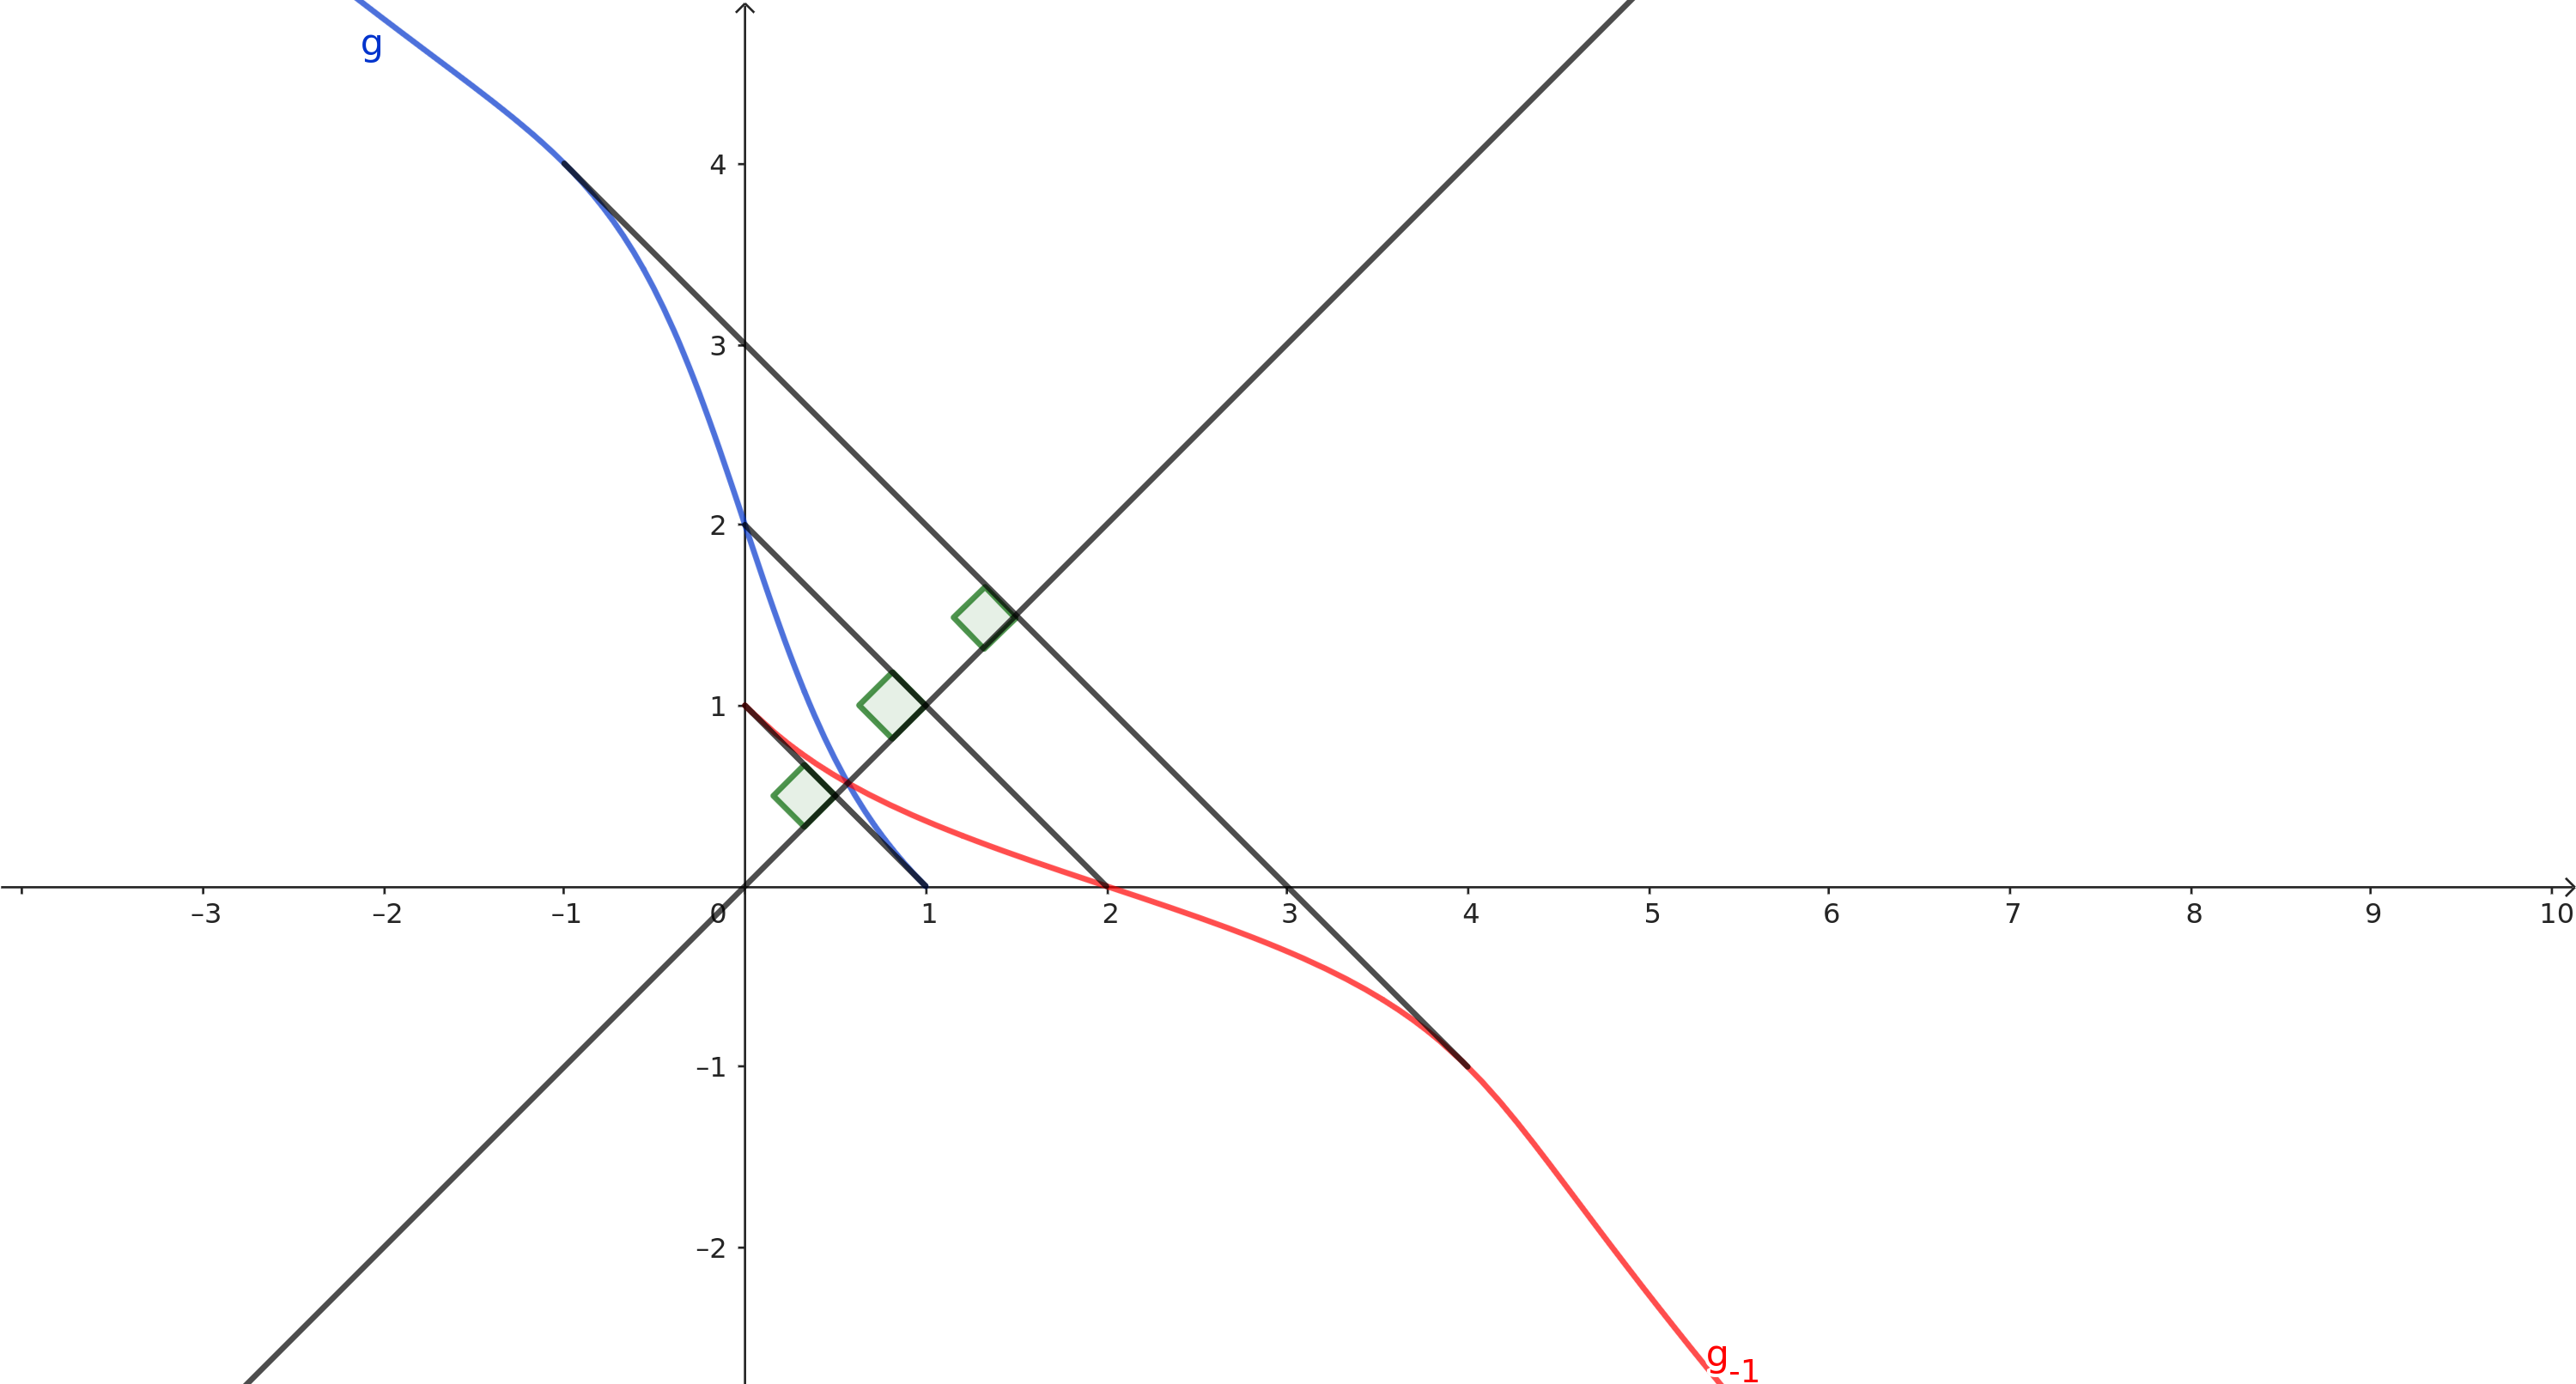
\includegraphics[width=0.8\textwidth]{Probleme1.png}
\caption{Courbe de (Cf)}
\label{fig:monimage}
\end{figure}
\href{https://www.geogebra.org/classic/tabyrtxt}{Clique ici pour voir la figure sur géogébra}
\section*{Problème n°2}

Soit la fonction numérique \( f : \mathbb{R} \to \mathbb{R} \) telle que :
\[
f(x) = 
\begin{cases} 
\frac{x - 1 + \sqrt{x^2 - x}}{x - 2} & \text{si } x \geq 1 \\
\frac{x - 1}{x^2 - 4x + 3} & \text{si } x < 1 
\end{cases}
\]

On désigne par \( (C_f) \) sa courbe représentative.

\subsection*{Partie A}

\begin{enumerate}
    \item Déterminer le domaine de définition de $f$.
    \item Calculer les limites aux bornes de $D_f$.
    \item Étudier la continuité de $f$ en 1.
    \item Étudier la dérivabilité de $f$ en 1. Interpréter graphiquement les résultats.
    \item 
    \begin{enumerate}
        \item Déterminer les réels $a$, $b$, et $c$ tels que : $f(x) = ax + b + \frac{c}{x-2}$, $\forall x < 1$.
        \item En déduire que $(C_f)$ admet au voisinage de $-\infty$ une asymptote oblique $(\Delta)$ dont on précisera son équation.
        \item Étudier la position relative de $(C_f)$ par rapport à $(\Delta)$ sur ]$-\infty ; 1[$.
    \end{enumerate}
    \item Étudier la nature de la branche infinie de $(C_f)$ au voisinage de $+\infty$, puis étudier sa position relative par rapport à $(C_f)$ s'il s'agit d'une asymptote.
    \item Déterminer $f'(x)$ sur chaque intervalle où $f$ est dérivable, puis en déduire son signe.
    \item Dresser le tableau de variation de $f$.
\end{enumerate}

\subsection*{Partie B}


Soit $h$ la restriction de $f$ à l’intervalle $I = ]-\infty; 1[$.
\begin{enumerate}
    \item Montrer que $h$ réalise une bijection de $I$ vers un intervalle $J$ à préciser.
    \item 
    \begin{enumerate}
        \item Calculer $h(0)$.
        \item $h^{-1}$ est-elle dérivable en $-\frac{3}{2}$ ? Si oui, déterminer $(h^{-1})'\left(-\frac{3}{2}\right)$.
        \item Déterminer le sens de variation de $h^{-1}$ puis dresser son tableau de variation.
    \end{enumerate}
    \item Déterminer l’expression de $h^{-1}(x)$.
    \item Tracer soigneusement $(C_f)$ et $(C_{h^{-1}})$ dans un repère orthonormé.
\end{enumerate}

\section*{Problème n°3}

\subsection*{\underline{Étude graphique}}
Soit $f$ une fonction dont la courbe représentative est donnée ci-dessous
\begin{figure}[H]% Forcer l'image à cet endroit
\centering
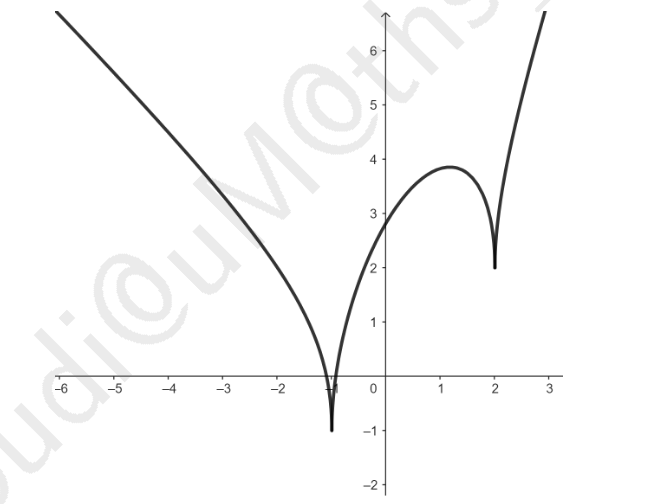
\includegraphics[width=0.8\textwidth]{graphe.png}
\caption{Courbe de (Cf)}
\label{fig:monimage}
\end{figure}
\begin{enumerate}
    \item Déterminer $f(-1)$ ; $f(2)$ et $D_f$.
    \item Déterminer les limites de $f$ aux bornes de $D_f$.
    \item 
    \begin{enumerate}
        \item $f$ est-elle dérivable en $-1$ et en $2$ ?
        \item Déterminer les variations de $f$ sur $]-\infty, -1[$ et sur $]2, +\infty[$.
    \end{enumerate}
\end{enumerate}

\subsection*{\underline{Étude numérique}}

Dans cette partie, on prend $f(x) = x + 2\sqrt{|x^2 - x - 2|}$.

\begin{enumerate}
    \item 
\begin{enumerate}
		\item[(a)] Déterminer le domaine de définition de $f$.
    \item[(b)] Écrire $f(x)$ sans symbole de la valeur absolue puis calculer les limites aux bornes de $D_f$.
    \item[(c)] Montrer que $(C_f)$ admet une asymptote oblique $(D)$ en $+\infty$ et donner l’équation de cette asymptote.
    \item[(d)] Étudier la position de $(C_f)$ par rapport à $(D)$.
    \item[(e)] Préciser la nature de l’asymptote à $(C_f)$ en $-\infty$.
\end{enumerate}

\item
\begin{enumerate}
    \item[(a)] Étudier la dérivabilité de $f$ en $-1$ et $2$. Interpréter le résultat obtenu.
    \item[(b)] Donner l’ensemble de dérivabilité de $f$ puis calculer $f'(x)$.
    \item[(c)] Démontrer que $f'(x) > 0$ sur $]2; +\infty[$ et que $f'(x) < 0$ sur $]-\infty; -1[$.
    \item[(d)] Résoudre l’inéquation $\sqrt{-x^2 + x + 2} \leq 2x - 1$ sur $]-1; 2[$.
    \item[(e)] Dresser le tableau de variation de $f$.
\end{enumerate}

\item
\begin{enumerate}
    \item[(a)] Soit $g$ la restriction de $f$ sur $I = ]2; +\infty[$. Montrer que $g$ est une bijection de $I$ sur $I$.
    \item[(b)] En étudiant la fonction $h$ définie par $h(x) = x - g(x)$, montrer qu’il existe un réel $\alpha$ vérifiant $g(\alpha) = \alpha$.
    \item[(c)] Déterminer par le calcul la valeur exacte de $\alpha$, puis déterminer $(g^{-1})(\alpha)$ si possible.
    \item[(d)] Tracer dans le même repère $(Cg)$ et $(Cg^{-1})$.
\end{enumerate}
\end{enumerate}
\section*{Problème n°4}
Soit $f$ la fonction définie par :
\[
f(x) =
\begin{cases}
-x + \sqrt{x^2 + 4} & \text{si } x < 0 \\
\sqrt{|4 - x^2|} & \text{si } x \geq 0
\end{cases}
\]

On note $(C_f)$ sa courbe représentative dans un repère orthonormé $(O, \vec{i}, \vec{j})$.

\begin{enumerate}
    \item Déterminer l’ensemble de définition de $f$.
    \item Écrire $f(x)$ sans le symbole de la valeur absolue.
    \item
    \begin{enumerate}
        \item Étudier la continuité de $f$ en 0.
        \item Étudier la dérivabilité de $f$ en 0. Interpréter les résultats.
        \item Étudier la dérivabilité de $f$ en 2. Interpréter les résultats.
    \end{enumerate}
    \item
    \begin{enumerate}
        \item Calculer les limites aux bornes de $D_f$.
        \item Étudier les branches infinies de $(C_f)$.
    \end{enumerate}
    \item On pose pour tout $x \in [0, 2]$, $h(x) = f(x) - x$.
    \begin{enumerate}
        \item Montrer que l’équation $h(x) = 0$ admet une unique solution notée $\alpha$.
        \item Vérifier que $\alpha \in \left[1, \frac{3}{2}\right]$.
    \end{enumerate}
    \item
    \begin{enumerate}
        \item Calculer $f'(x)$ sur chaque intervalle où $f$ est dérivable.
        \item Dresser le tableau de variations de $f$.
        \item[(c)] Construire $(C_f)$.
    \end{enumerate}
    \item[7.] Soit $g$ la restriction de $f$ sur $I = ]2; +\infty[$.
    \begin{enumerate}
        \item Montrer que $g$ est une bijection de $I$ vers un intervalle $J$ à préciser.
        \item Montrer que $g^{-1}$ est dérivable en $\sqrt{5}$ puis calculer $(g^{-1})'(\sqrt{5})$.
        \item Expliciter $g^{-1}(x)$.
        \item Tracer $(C_{g^{-1}})$ dans le même repère que $(C_f)$.
    \end{enumerate}
    \item[8.] Montrer que pour tout $x \in \left[ 1, \frac{3}{2} \right]$, $|f'(x)| \leq \frac{3\sqrt{7}}{7}$.
    \item[9.] En déduire que $|f(x) - \alpha| \leq \frac{3\sqrt{7}}{7} |x - \alpha|$, pour tout $x \in \left[ 1, \frac{3}{2} \right]$.
\end{enumerate}
\end{document}
